
% This LaTeX was auto-generated from MATLAB code.
% To make changes, update the MATLAB code and republish this document.











    
    \begin{DoxyCode}
function example_dirac()
\end{DoxyCode}
\begin{par}
COMPILATION
\end{par} \vspace{1em}
\begin{DoxyCode}
    [exdir,~,~]=fileparts(which('example_dirac.m'));
    % compile the model
    amiwrap('model_dirac','model_dirac_syms',exdir)
\end{DoxyCode}

         \begin{DoxyCode}Generating model struct ...
Parsing model struct ...

Generating C code ...
headers | wrapfunctions | 
Compiling mex file ...
amici | Building with 'Xcode with Clang'.
MEX completed successfully.
Building with 'Xcode with Clang'.
MEX completed successfully.
\end{DoxyCode} 
    \begin{par}
SIMULATION
\end{par} \vspace{1em}
\begin{DoxyCode}
    % time vector
    t = linspace(0,3,1001);
    p = [1;0.5;2;3];
    k = [];

    options = amioption('sensi',0,...
        'maxsteps',1e4);

    % load mex into memory
    [msg] = which('simulate_model_dirac'); % fix for inaccessability problems
    sol = simulate_model_dirac(t,log10(p),k,[],options);

    tic
    sol = simulate_model_dirac(t,log10(p),k,[],options);
    disp(['Time elapsed with amiwrap: ' num2str(toc) ])
\end{DoxyCode}

         \begin{DoxyCode}Time elapsed with amiwrap: 0.0045507
\end{DoxyCode} 
    \begin{par}
ODE15S
\end{par} \vspace{1em}
\begin{DoxyCode}
    sig = 1e-2;
    delta_num = @(tau) exp(-1/2*(tau/sig).^2)/(sqrt(2*pi)*sig);

    ode_system = @(t,x,p,k) [-p(1)*x(1)+delta_num(t-p(2));
        +p(3)*x(1) - p(4)*x(2)];

    options_ode45 = odeset('RelTol',options.rtol,'AbsTol',options.atol,'MaxStep',options.maxsteps);

    tic
    [~, X_ode45] = ode45(@(t,x) ode_system(t,x,p,k),t,[0;0],options_ode45);
    disp(['Time elapsed with ode45: ' num2str(toc) ])
\end{DoxyCode}

         \begin{DoxyCode}Time elapsed with ode45: 0.080371
\end{DoxyCode} 
    \begin{par}
PLOTTING
\end{par} \vspace{1em}
\begin{DoxyCode}
    figure
    c_x = get(gca,'ColorOrder');
    subplot(2,2,1)
    for ix = 1:size(sol.x,2)
        plot(t,sol.x(:,ix),'.-','Color',c_x(ix,:))
        hold on
        plot(t,X_ode45(:,ix),'--','Color',c_x(ix,:))
    end

    legend('x1','x1_{ode45}','x2','x2_{ode15s}','Location','NorthEastOutside')
    legend boxoff
    xlabel('time t')
    ylabel('x')
    box on
    subplot(2,2,2)
    plot(t,abs(sol.x-X_ode45),'--')
    set(gca,'YScale','log')
    ylim([1e-10,1e0])
    legend('error x1','error x2','Location','NorthEastOutside')
    legend boxoff

    subplot(2,2,3)
    plot(t,sol.y,'.-','Color',c_x(1,:))
    hold on
    plot(t,X_ode45(:,2),'--','Color',c_x(1,:))
    legend('y1','y1_{ode45}','Location','NorthEastOutside')
    legend boxoff
    xlabel('time t')
    ylabel('y')
    box on

    subplot(2,2,4)
    plot(t,abs(sol.y-X_ode45(:,2)),'--')
    set(gca,'YScale','log')
    ylim([1e-10,1e0])
    legend('error y1','Location','NorthEastOutside')
    legend boxoff
    xlabel('time t')
    ylabel('y')
    box on
    set(gcf,'Position',[100 300 1200 500])
\end{DoxyCode}

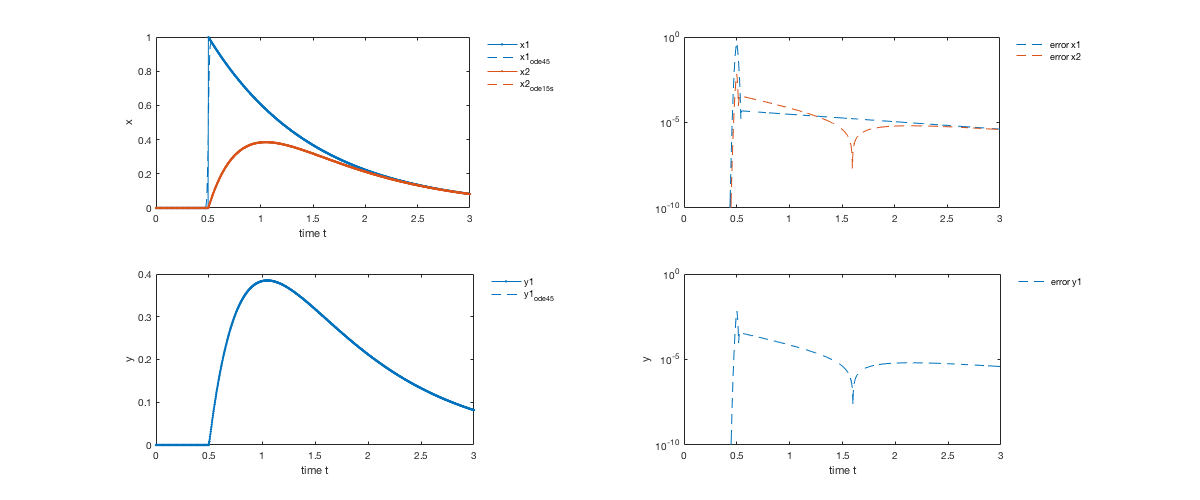
\includegraphics[width=\textwidth]{../../examples/example_dirac/html/example_dirac_01.png}
\begin{par}
FORWARD SENSITIVITY ANALYSIS
\end{par} \vspace{1em}
\begin{DoxyCode}
    options.sensi = 1;

    sol = simulate_model_dirac(t,log10(p),k,[],options);
\end{DoxyCode}
\begin{par}
FINITE DIFFERENCES
\end{par} \vspace{1em}
\begin{DoxyCode}
    eps = 1e-4;
    xi = log10(p);
    for ip = 1:4;
        xip = xi;
        xip(ip) = xip(ip) + eps;
        solp = simulate_model_dirac(t,xip,k,[],options);
        sx_fd(:,:,ip) = (solp.x - sol.x)/eps;
        sy_fd(:,:,ip) = (solp.y - sol.y)/eps;
    end
\end{DoxyCode}
\begin{par}
PLOTTING
\end{par} \vspace{1em}
\begin{DoxyCode}
    figure
    for ip = 1:4
        subplot(4,2,ip*2-1)
        hold on
        for ix = 1:size(sol.x,2)
            plot(t,sol.sx(:,ix,ip),'.-','Color',c_x(ix,:))
            plot(t,sx_fd(:,ix,ip),'--','Color',c_x(ix,:))
        end
        ylim([-2,2])
        legend('x1','x1_{fd}','x2','x2_{fd}','Location','NorthEastOutside')
        legend boxoff
        title(['state sensitivity for p' num2str(ip)])
        xlabel('time t')
        ylabel('x')
        box on

        subplot(4,2,ip*2)
        plot(t,abs(sol.sx(:,:,ip)-sx_fd(:,:,ip)),'r--')
        legend('error x1','error x2','Location','NorthEastOutside')
        legend boxoff
        title(['state sensitivity for p' num2str(ip)])
        xlabel('time t')
        ylabel('error')
        ylim([1e-12,1e0])
        set(gca,'YScale','log')
        box on
    end
    set(gcf,'Position',[100 300 1200 500])

    figure
    for ip = 1:4
        subplot(4,2,ip*2-1)
        hold on
        for iy = 1:size(sol.y,2)
            plot(t,sol.sy(:,iy,ip),'.-','Color',c_x(iy,:))
            plot(t,sy_fd(:,iy,ip),'--','Color',c_x(iy,:))
        end
        ylim([-2,2])
        legend('y1','y1_{fd}','Location','NorthEastOutside')
        legend boxoff
        title(['observable sensitivity for p' num2str(ip)])
        xlabel('time t')
        ylabel('y')
        box on

        subplot(4,2,ip*2)
        plot(t,abs(sol.sy(:,:,ip)-sy_fd(:,:,ip)),'r--')
        legend('error y1','Location','NorthEastOutside')
        legend boxoff
        title(['observable sensitivity for p' num2str(ip)])
        xlabel('time t')
        ylabel('error')
        ylim([1e-12,1e0])
        set(gca,'YScale','log')
        box on
    end
    set(gcf,'Position',[100 300 1200 500])

    drawnow
\end{DoxyCode}

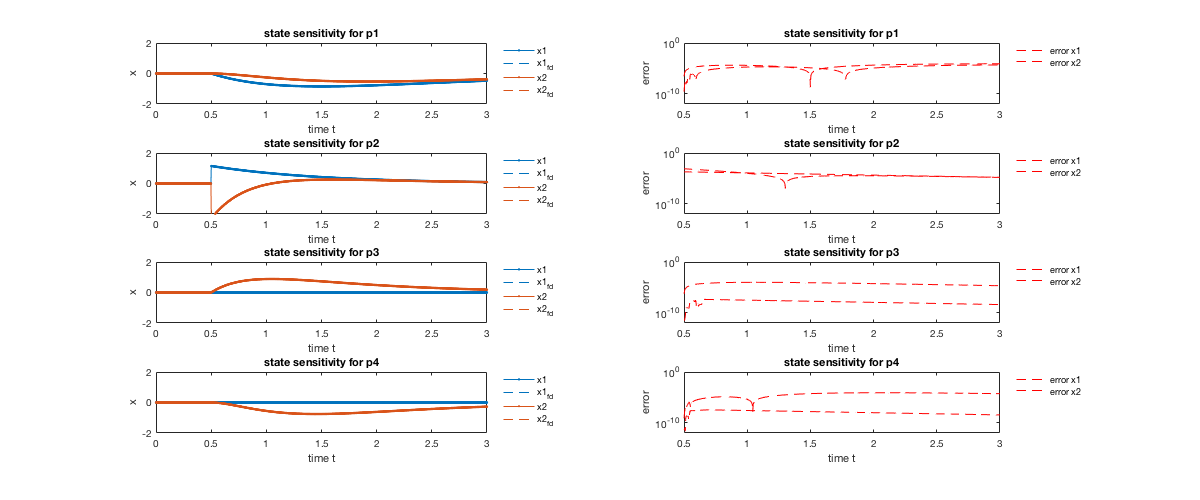
\includegraphics[width=\textwidth]{../../examples/example_dirac/html/example_dirac_02.png}

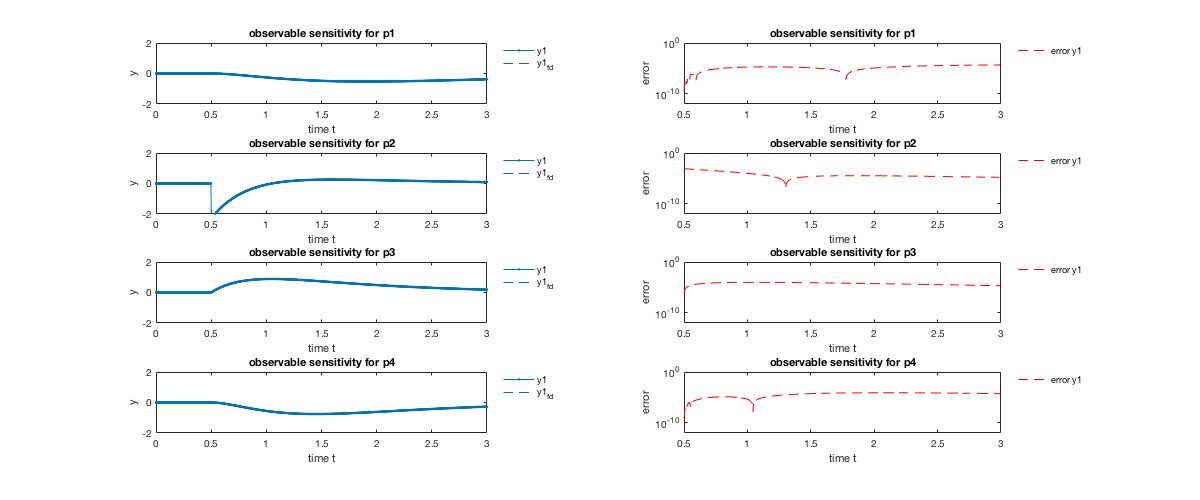
\includegraphics[width=\textwidth]{../../examples/example_dirac/html/example_dirac_03.png}
\begin{DoxyCode}
end
\end{DoxyCode}




    